\documentclass[numbers=noenddot,14pt,a4paper]{scrartcl}
\usepackage[greek,ngerman]{babel}
\usepackage[T1]{fontenc}
\usepackage[utf8]{inputenc}
\usepackage{fullpage}
\usepackage{libertine}
\usepackage{ziffer}
\usepackage{graphicx}
\usepackage{units}
\usepackage[infoshow]{tabularx}
\usepackage{amsmath}
\usepackage{amssymb}
\usepackage{wrapfig}
\usepackage{esint}
\usepackage{float}
\usepackage{wrapfig}
\usepackage[font=small]{caption}
\usepackage{subcaption}
\usepackage{lscape}
\usepackage{hyperref}

\renewcommand{\thefigure}{Abb. \arabic{figure}}

\captionsetup[wrapfigure]{name=}
\captionsetup[figure]{name=}
\newcommand{\degree}{^\circ}
\newcommand{\diff}{\textnormal{d}}
\newcommand{\tenpo}[1]{\cdot 10^{#1}}
\newcommand{\greek}[1]{\greektext#1\latintext}
\newcommand{\ix}[1]{_\text{#1}}
\newcommand{\imag}{\mathbf{i}}
\newcommand{\tilt}[1]{\textit{#1}}
\newcommand{\grad}[1]{\textit{grad}\left(#1\right)}
\newcommand{\divergenz}[1]{\textit{div}\left(#1\right)}
\newcommand{\euler}{\mathnormal{e}}
\newcommand{\fett}[1]{\textbf{#1}}

\title{Protokoll: Hall-Effekt in Halbleitern} %TODO Name des Versuchs eintragen
\author{Tom Kranz, \underline{Philipp Hacker}}
\date{\today}

\begin{document}
%\setcounter{page}{2}
%\setcounter{section}{1}
\maketitle
\begin{center}
Betreuer: Dr. Marvin von der Ehe\\ %TODO Name des Betreuers eintragen
Versuchsdatum: 18.11.2014\\ %TODO Datum des Versuchs eintragen
\begin{table}[h]
\centering
Note: %TODO Gute Note erhalten :)
\begin{tabularx}{1.5cm}{|X|}
\hline \\ \\
\hline
\end{tabularx}
\end{table}
\end{center}
\vspace*{\fill}
\tableofcontents
\vfill
\newpage
\section{Einleitung}
Dem sog. \tilt{Hall-Effekt} bedient man sich bei der Messung von magnetischen Feldstärken. Dabei werden Halbleiter eingesetzt, die in ihren attraktiven Eigenschaften sich dafür sehr gut eignen. In diesem Versuch sollen die Prinzipien dieser Vorgehensweise und die Unterschiede zwischen verschieden \tilt{dotierten} Materialien aufgezeigt werden. Im Fokus stehen außerdem die Untersuchungen von Beweglichkeit der Ladungsträger, der Konzentrationen dieser und deren Rückschlüsse auf interne Stromflussprozesse im Halbleiter.
\section{Physikalische Grundlagen}
\subsection{Halbleiter}
\begin{wrapfigure}[15]{ro}{0.5\textwidth}
	\includegraphics[width=0.5\textwidth]{Bandstruktur_GaAs.png}
	\caption{reduzierte Bandstruktur in Silizium mit eingezeichneten Richtungsachsen}
	 \label{img:band}
\end{wrapfigure}
Halbleiter sind Festkörper, welche sich durch eine kleine, nicht von Ladungsträgern besiedelten Energielücke $E\ix{G}$ zwischen dem letzten besetzen Energieband, dem \tilt{Valenzband}, und dem darauf folgendem, dem \tilt{Leitungsband} charakterisieren (\ref{img:band}). Nach \tilt{Wolfgang Pauli} (1925) kann das $N$-te Band maximal mit $2N$ verschiedenen Zuständen der Ladungsträger, den Elektronen besetzt werden. Diese werden in, an die Atome im Gitter des Halbleiter-Kristalls gebundene Rumpfelektronen und quasifreie, bewegliche Elektronen unterschieden.\\
In Halbleiter können damit bereits durch thermische Anregung oder kleine äußere Felder Elektronen in das Leitungsband übergehen und damit einen elektrischen Strom fließen lassen. Aus dem Übergang geht auch ein sog. \tilt{Defektelektron} hervor, was einen unbesetzten Zustand oder ein Loch im Band, aus welchen das Elektronen abwandert, ausdrückt und damit die Gleichheit von Loch- und Ladungsträgerkonzentration fordert. Diese wird als \tilt{intrinsische Ladungsträgerdichte} bezeichnet. Der entstehende Strom heißt \tilt{Rekombinationsstrom}, da er durch die \tilt{Rekombination} eines Elektron-Loch-Paares charakterisiert wird. Es sei angemerkt, dass die Bewegung der Elektronen, quantenmechanisch betrachtet, durch eine Welle mit Richtungsvektor $\vec{k}$ und der Winkelgeschwindigkeit $\omega$ ausgedrückt werden kann.\\
Betrachtet man die Defektelektronen als pos. Ladungen, so tragen sie unter einen äußeren elektrischen Feld $\vec{E}$ zu der Dichte des dabei fließenden Stromes $\vec{j}$ aus Gl. (\ref{eq:strom}) bei. Hierbei haben die Quasi"~/Teilchen einmal die Geschwindigkeit $\vec{v}\ix{n/p}$. Diese Eigenschaft nennt man \tilt{Eigentleitung} $\sigma\ix{i}$. Allgemein sind jedoch die Beweglichkeiten $\mu$ und Konzentrationen $p$ bzw. $n$ von Löchern und freien Elektronen nicht gleich (Verunreinigungen).
\begin{align}
	\vec{j}=q\ix{e}n\vec{v}\ix{n}+q\ix{p}p\vec{v}\ix{p}=e\left(n\mu\ix{n}+p\mu\ix{p}\right)\vec{E}=\sigma\vec{E} \label{eq:strom}
\end{align}
($\sigma$ - Leitfägikeit; $e$ - Elementarladung; $q\ix{i}$ - Ladung der Teilchen)
\subsection{Ladungsträgerdichten und Beweglichkeiten}
\subsubsection{Ladungsträgerdichten}
Da eine thermische  bzw. äußere Anregung nötig ist, um Elektronen ins Leitungsband zu bewegen, kann eine starke Temperaturabhängigkeit von $n$ und $p$ gefolgert werden. Die Besetzung der Energieniveaus muss der Fermi-Statistik $f\left(E,T\right)$ folgen. In der Regel ist jedoch die Aufweichung von $f\left(E,T\right)$ im Bereich $\sim2k\ix{B}T$ und damit sehr klein gegen $E\ix{G}$. Sie kann deswegen durch die Boltzmann-Statistik ersetzt werden, sofern $E-E\ix{F}>>2k\ix{B}T$ für die Fermi-Energie zwischen den Bändern gilt. Damit werden die Ladungsträgerdichten zu:
\begin{align}
	n=&\int_{E\ix{L}}^{\infty}D\ix{L}\left(E\right)\euler^{-\frac{E-E\ix{F}}{k\ix{B}T}}\diff E=\int_{E\ix{L}}^{\infty}\frac{\left(2m\ix{n}\right)^{3/2}}{2\pi^2\hbar^3}\sqrt{E-E\ix{L}}\euler^{-\frac{E-E\ix{F}}{k\ix{B}T}}\diff E \nonumber \\
	=&\frac{\left(2m\ix{n}k\ix{B}T\right)^{3/2}}{2\pi^2\hbar^3}\euler^{-\frac{E\ix{L}-E\ix{F}}{k\ix{B}T}}\int_{E\ix{L}}^{\infty}\sqrt{E-E\ix{L}}\euler^{-\frac{E}{k\ix{B}T}}\diff E \nonumber \\
	=&2\left(\frac{2\pi m\ix{n}k\ix{B}T}{h^2}\right)^{3/2}\euler^{-\frac{E-E\ix{F}}{k\ix{B}T}}=N^L\ix{eff}\euler^{-\frac{E\ix{L}-E\ix{F}}{k\ix{B}T}} \\
	\text{analog} \, \,\, p=&2\left(\frac{2\pi m\ix{p}k\ix{B}T}{h^2}\right)^{3/2}\euler^{-\frac{E\ix{V}-E\ix{F}}{k\ix{B}T}}=N^V\ix{eff}\euler^{-\frac{E\ix{V}-E\ix{F}}{k\ix{B}T}}
\end{align}
($D\ix{L/V}$ - Zustandsdichten in den Bändern; $m\ix{n/p}$ - effektive Massen; $E\ix{V}$,$E\ix{L}$ - Bandkanten)\\
Die Konzentrationen für quasifreie Ladungsträger folgen somit der Boltzmann-Statistik. Die Faktoren $N^{L/V}\ix{eff}$ sind die effektiven Zustandsdichten und gehen mit $T^{3/2}$. Man kann nun sich das jeweilige Band als ein einziges Energieniveau mit den betreffenden Zustandsdichten denken. Die Besetzungsdichte wird durch die Boltzmann-Verteilung geregelt. Beachtet werden muss jedoch, das ebenso $E\ix{F}$ als auch $E\ix{V/L}$ von außen verschoben werden können. Dem folgen die Integrale der Besetzungsdichten nach. Außerdem ist offensichtlich $E\ix{G}=E\ix{L}-E\ix{V}$.\\
Die besprochene intrinsische Ladungsträgerkonzentration wird damit zu
\begin{align}
	n\ix{i}=\sqrt{np}=\sqrt{4\left(\frac{k\ix{B}T}{2\pi\hbar^2}\right)^3\left(m\ix{n}m\ix{p}\right)^{3/2}\euler^{-\frac{E\ix{G}}{k\ix{B}T}}}=\sqrt{N^{V}\ix{eff}N^{L}\ix{eff}}\euler^{-\frac{E\ix{G}}{2k\ix{B}T}} \label{eq:intrin}
\end{align}
Bei geeigneter Handhabung der Messwerte, sowie einigen Näherungen bezüglich der Verhältnisse der Ladungsträgerkonzentrationen, kann man durch Gl. (\ref{eq:logsigma}) die Bandlücke bestimmen.
\begin{align}
	\sigma\ix{i}=&e\left(n\ix{i}\mu\ix{n}+n\ix{i}\mu\ix{p}\right)=en\ix{i}\left(\mu\ix{p}+\mu\ix{n}\right) \nonumber \\
	\ln{\left(\sigma\ix{i}\right)}=&\ln{\left(\sqrt{N^{V}\ix{eff}N^{L}\ix{eff}}\left(\mu\ix{n}+\mu\ix{p}\right)\right)}-\frac{E\ix{G}}{2k\ix{B}T} \nonumber \\
	=&\frac{1}{2}\left(\ln\left(N^{V}\ix{eff}\right)+\ln\left(N^{L}\ix{eff}\right)\right)+\ln\left(\mu\ix{n}\right)\ln\left(\mu\ix{p}\right)-\frac{E\ix{G}}{2k\ix{B}T} \label{eq:logsigma} \\
	\hat{=}&\,a\cdot x+b \nonumber \\
	\text{mit} \,\,\, x=&\frac{1}{T} \,\,;\,\, a=\frac{E\ix{G}}{2k\ix{B}} \,\,;\,\, b=\frac{1}{2}\left(\ln\left(N^{V}\ix{eff}\right)+\ln\left(N^{L}\ix{eff}\right)\right)+\ln\left(\mu\ix{n}\right)\ln\left(\mu\ix{p}\right) \nonumber
\end{align}
\subsubsection{Beweglichkeiten}
Die Beweglichkeiten $\mu\ix{n/p}$ sind Mittelwerte über die besetzten Zustände im Valenz- und Leitungsband. Löcher und Elektronen verhalten sich dabei qualitativ gleich. Es gilt wiederum die Boltzmann-Statistik für die folgenden Mittelwerte ($\tau(\vec{k})$ - Relaxationszeit  des Elektrons am reziproken "`Ort"' $\vec{k}$).
\begin{align}
	\mu=\frac{1}{m}\frac{\langle\tau(\vec{k}) v^2(\vec{k})\rangle}{\langle v^2(\vec{k})\rangle}
\end{align}
Grob kann gefolgert werden, dass $\mu\sim\tau$. Jedoch ist $\tau$ proportional zur mittleren freien Weglänge der bewegten Ladungsträger. Somit kann man $\frac{1}{\tau}\sim\langle v\rangle\Sigma$ für einen Streuquerschnitt der Teilchen $\Sigma$ als Stoßwahrscheinlichkeit auffassen. Außerdem ist, wegen der Boltzmann-Statistik der Bewegungen \mbox{$\langle v\rangle\sim\sqrt{T}$.} Nimmt man nun an, das die Streuung nur an Phononen oder ionisierten Störstellen stattfindet kann, so folgen 2 grundlegende Überlegungen:
\begin{itemize}
	\item{der Streuquerschnitt eines Phonons mit ($\vec{q},\omega(\vec{q}))$ sei $\Sigma\ix{Ph}$, so kann man für $T<<\Theta\ix{Deb}$ annehmen:}
	\begin{align}
		\Sigma\ix{Ph}\sim m\cdot\omega^2(\vec{q})\cdot\langle s^2(\vec{q})\rangle\sim T \label{eq:phononen}
	\end{align}
	\item{für einen, an einer ionisierten Störstelle vorbeifliegenden Ladungsträger ist der Streuquerschnitt nach \tilt{Rutherford} $\Sigma\ix{St}\sim \langle v\rangle^4$, woraus mit der Störstellenkonzentration $N\ix{St}$ folgt:}
	\begin{align}
		\frac{1}{\tau\ix{St}}\sim \frac{N\ix{St}}{T^{3/2}} \label{eq:stör}
	\end{align}
\end{itemize}
Benutzt man jetzt die vorherigen Aussagen zusammen mit Gl (\ref{eq:phononen}) und (\ref{eq:stör}), so erhält man für die Beweglichkeit in verschiedene Temperaturbereichen (siehe \ref{img:beweglichkeit}):
\begin{align}
	\mu\ix{St}\sim T^{3/2} \,\, \text{und} \,\, \mu\ix{Ph}\sim T^{-3/2} \label{eq:beweg2}
\end{align}
Offensichtlich findet für große Temperaturen mehr Streuung an Phononen statt, da dort natürlich das mittlere Schwingungsquadrat des Gitters größer ist. Zudem folgt dies ebenso aus den Voraussetzungen von Gl. (\ref{eq:phononen}). Für kleinere Temperaturen mit $T<<\Theta\ix{Deb}$ überwiegt die Ablenkung durch die Coulomb-Abstoßung an Störstellen mit Ladungen.
\begin{figure}[H]
	\centering
	\includegraphics[width=0.6\textwidth]{beweglichkeit.png}
	\caption{Doppeltlogarithmische Auftragung der Beweglichkeit über die Temperatur}
	\label{img:beweglichkeit}
\end{figure}
\subsection{Dotierter Halbleiter}\label{ch:dot}
Den Einbau von Fremdatomen unterschiedlicher Wertigkeiten (im Vergleich zum Material des Halbleiters) bezeichnet man als Dotierung. Diese ist gleichzusetzen mit dem künstlichen Erzeugen von freien Elektronen bzw. Defekten. Man verändert folglich die Konzentration der Ladungsträger, was Einfluss auf Leitfähigkeit und thermisches Verhalten hat. Die Donatoren (größere Wertigkeit) und Akzeptoren (kleinere Wertigkeit) verändern die Bandstruktur und explizit die Bandlücke des Halbleiterkristalls, indem sie in ihren unterschiedlichen Energieniveaus Defekt-/Elektronen abgeben bzw. aufnehmen. Dadurch reichen schon geringere Anregungsenergien der Ladungsträger aus, damit sie im Leitungsband zum Strom beitragen können. Etwas genauer heißt das, dass Akzeptoren die obere Bandkante ($E\ix{L}$) herabsetzen und Donatoren die untere ($E\ix{V}$) anheben. Dotiert man einen Kristall mit nur einer Sorte von Fremdatomen, so spricht man entweder von einem p-dotierten (für Akzeptoren) oder n-dotierten (für Donatoren) Halbleiter.\\
Die Annahme gleicher Konzentrationen $n$ und $p$ kann, wie angesprochen, nicht mehr gelten. Deswegen führt man mit den Dichten der neutralen ($N\ix{D}^{0}$)  und ionisierten ($N\ix{D}^{+}$) Donatoren (analog Akzeptoren) die folgenden Ladungsträgerdichten ein:
\begin{align}
	N\ix{D}=&N\ix{D}^0+N\ix{D}^+ \label{eq:donator}\\
	N\ix{A}=&N\ix{A}^0+N\ix{A}^- \,\,.
\end{align}
Hierbei wurde beachtet, das ionisierte Akzeptoren negativ und Donatoren positiv geladen werden, falls sie zur sog. \tilt{Störstellenleitung} beitragen.\\
Aufgrund der Ladungsneutralität im gesamten Halbleiter muss \mbox{$n+N\ix{A}^-=p+N\ix{D}^+$} gelten. Für die Besetzung $n\ix{D}$ bzw. $p\ix{A}$ der jeweiligen Fremdatome kann man die Fermi-Statistik benutzen.
\begin{align}
	n\ix{D}=N\ix{D}^0=N\ix{D}\left(\frac{1}{1+\euler^{\frac{E\ix{D}-E\ix{F}}{k\ix{B}T}}}\right) \,\,\, \text{und} \,\,\, p\ix{A}=N\ix{A}^0=N\ix{A}\left(\frac{1}{1+\euler^{\frac{E\ix{F}-E\ix{A}}{k\ix{B}T}}}\right) \label{eq:besetzungdot}
\end{align}
($E\ix{A/D}$ - Energieniveaus der Dotierungen)\\
Nimmt man an, dass ein reiner n-Halbleiter vorliegt und dass der größte Beitrag zur Leitfähigkeit von den Donatoren geleistet wird ($N\ix{D}^+>>n\ix{i}$), so kann man unter Verwendung von Gln. (\ref{eq:besetzungdot}), (\ref{eq:donator})  und (\ref{eq:intrin}) schreiben:
\begin{align}
	n=N\ix{D}^++p\approx N\ix{D}^+=N\ix{D}-N\ix{D}^0\approx& N\ix{D}\left(1-\frac{1}{1+\euler^{\frac{E\ix{D}-E\ix{F}}{k\ix{B}T}}}\right) \nonumber \\
	\left(\euler^{\frac{E\ix{F}}{k\ix{B}T}}=\frac{n}{N\ix{eff}^L}\euler^{\frac{E\ix{L}}{k\ix{B}T}} \,\,\,;\,\,\, E\ix{d}=E\ix{L}-E\ix{D}\right) \Rightarrow \,\,\,\approx& \frac{N\ix{D}}{1+\frac{n}{N\ix{eff}^L}\euler^{\frac{E\ix{d}}{k\ix{B}T}}} \label{eq:konzentration2}
\end{align}
Nach Umstellen von Gl. (\ref{eq:konzentration2}) folgt Gl. (\ref{eq:konzentration}).
\begin{align}
	n\approx 2N\ix{D}\left(1+\sqrt{1+4\frac{N\ix{D}}{N\ix{eff}^L}\euler^{\frac{
		E\ix{D}}{k\ix{B}T}}}\right)^{-1} \label{eq:konzentration}
\end{align}
Gleichung (\ref{eq:konzentration}) lässt sich qualitativ für verschiedene Grenzfälle diskutierten (siehe \ref{img:schemakonzentration}):
\begin{itemize}
	\item[$\euler^\frac{E\ix{d}}{k\ix{B}T}\rightarrow\infty$:]
		{Es sind so wenige Ladungsträger angeregt, dass $n<<n\ix{D}$ ist. Alle von den Donatoren abgegebenen Elektronen werden kompensiert (Kompensationsbereich).}
	\item[$\euler^\frac{E\ix{d}}{k\ix{B}T}>>1$:]
		{Hier gilt die sog. Störstellenreserve - viele Donatoren sind noch nicht ionisiert. Die Ladungsträgerkonzentration geht wie die des intrinsischen Halbleiters nach Gl. (\ref{eq:intrin}) mit $E\ix{d}$.}
	\item[$E\ix{d}\leq k\ix{B}T$:]
		{Alle Donatoren sind ionisiert und die Ladungsträgerkonzentration ist $n=N\ix{D}=const.\,$ Im Störstellenerschöpfungszustand spielen Valenzband-Elektronen für $n$ keine Rolle.}
	\item[$T\rightarrow\infty$:]
		{Für sehr große Temperaturen überwiegen die thermisch angeregten Elektronen aus dem Valenz-Band die Donator-Ladungsträger. Die gemachten Näherungen für Gl. (\ref{eq:konzentration}) sind nicht mehr gültig. Man spricht von Eigenleitung.}
\end{itemize}
\begin{figure}[H]
	\centering
	\includegraphics[width=0.8\textwidth]{temperaturverlaufkonzentration.png}
	\caption{Temperaturverlauf der Konzentration eines n-Halbleiters nach Gl. (\ref{eq:konzentration})} \label{img:schemakonzentration}
\end{figure}
\subsection{Hall-Effekt}
An einem Halbleiter, welcher senkrecht zum durchfließenden Strom von einem Magnetfeld durchsetzt wird, kann wiederum senkrecht auf Strom- und Magnetfeldrichtung eine Spannung gemessen werden. Diese ist die Hall-Spannung und wurde nach dem US-amerikanischen Physiker \tilt{Edwin Hall} benannt.\\
Aufgrund der Lorentz-Kraft $\vec{F}\ix{L}$ erfahren die Ladungsträger des Stromes $\vec{j}$ eine Ablenkung durch das Magnetfeld $\vec{B}$ senkrecht zu ihrer Bewegungsrichtung, welche der Richtung von $\vec{v}$ entspricht (Gl. (\ref{eq:lorentz})). Das Hall-Feld $\vec{E}\ix{H}$ wächst solange an, bis die dazugehörige Kraft $\vec{F}\ix{H}$ die Lorentz-Kraft kompensiert (Gl.(\ref{eq:lorentz})).
\begin{align}
	\vec{F}=\vec{F\ix{L}}+\vec{F}\ix{H}=\frac{1}{qn}\left(\vec{j}\times\vec{B}\right)+q\vec{E}\ix{H}=q\left(\vec{v}\times\vec{B}\right)+q\vec{E}\ix{H}=0 \label{eq:lorentz}
\end{align}
Weil für Defekte die Vorzeichenwechsel in $q$ und $\vec{v}$ sich gerade aufheben, folgt, dass Elektronen und Löcher durch den Hall-Effekt in die selbe Richtung bewegt werden. Die Hall-Spannung resultiert somit nur aus den Unterschieden zwischen den Konzentrationen und Beweglichkeiten der beiden Typen von Ladungsträgern. Offensichtlich ist sie deshalb eine geeignete Größe, um die genannten Charakteristiken zu messen.\\
Für einen Strom $\vec{j}=\left(j\ix{x},0,0\right)$ (aus einem ext. Feld $\vec{E}=\left(E\ix{x},0,0\right)$) und ein Magnetfeld $\vec{B}=\left(0,0,B\ix{z}\right)$ ist $\vec{E}\ix{H}=\left(0,E\ix{H},0\right)$.\\
Sei der Querschnitt des Leiters gerade $A=bd$, der Strom somit $I=j\ix{x}A$ und der Halbleiter entweder ein reiner p-/n-Leiter, so folgt für die Hall-Spannung $U\ix{H}$:
\begin{align}
U^n\ix{H}=-\frac{1}{ne}\frac{IB\ix{z}}{d}=R\ix{H}^n\frac{IB\ix{z}}{d} \,\,\, \text{und} \,\,\, U^p\ix{H}=\frac{1}{pe}\frac{IB\ix{z}}{d}=R\ix{H}^p\frac{IB\ix{z}}{d}
\end{align}
($R\ix{H}^{n/p}$ - Hall-Konstanten)\\
Allgemein liegen jedoch keine reinen n-/p-Halbleiter vor, weswegen eine weitere Betrachtung von $R\ix{H}$ notwendig wird.\\
Mit dem ohmschen Gesetz folgt für die Stromdichten $j\ix{y}$:
\begin{align}
	F^n=-e\left(v\ix{x}^nB+E\ix{H}\right)\,\,\, \text{und}\,\,\,	F^p=e\left(v\ix{x}^pB+E\ix{H}\right) \nonumber \\
	j\ix{y}^n=\sigma^n\frac{F^n}{(-e)}=n\mu\ix{n}e\left(E\ix{H}+v\ix{x}^nB\right)=n\mu\ix{n}e\left(E\ix{H}+\mu\ix{n}E\ix{x}B\right) \nonumber \\ \text{analog}\,\,\,j\ix{y}^p=p\mu\ix{p}e\left(E\ix{H}+\mu\ix{p}E\ix{x}B\right) \nonumber
\end{align}
Aufgrund der Ladungserhaltung muss die Summe der Ströme verschwinden. Äquivalent gilt dies für die Stromdichten. Stellt man diese Bedingung nach dem Hall-Feld $E\ix{H}$ um, so erhält man mit $E\ix{x}=\frac{j\ix{x}}{\sigma\ix{ges}}$
\begin{align}
	E\ix{H}=&\frac{e\left(\mu\ix{n}^2n-\mu\ix{p}^2p\right)}{\sigma\ix{ges}}E\ix{x}B=\frac{\mu\ix{n}^2n-\mu\ix{p}^2p}{n\mu\ix{n}+p\mu\ix{p}}E\ix{x}B \nonumber \\
	\text{und damit} \,\,\, R\ix{H}=&\frac{E\ix{H}}{j\ix{x}B}=\frac{\mu\ix{n}^2n-\mu\ix{p}^2p}{e\left(p\mu\ix{p}+n\mu\ix{n}\right)^2} \label{eq:hall-konst}
\end{align}
\newpage
\section{Durchführung}
\begin{wrapfigure}[17]{ro}{0.5\textwidth}
	\centering
	\includegraphics[width=0.5\textwidth]{aufbau.png}
	\caption{Oben: Hall-Sonde vor Kristallplatine\\Unten:Spulen-Paar auf Polschuhen}
\end{wrapfigure}
In diesem Versuch benutzten wir den Hall-Effekt um Untersuchungen zur Leitfähigkeit und damit der Beweglichkeit und Konzentration der Ladungsträger in Halbleitern zu machen. Grundlage bildete damit eine sog. Hall-Sonde, sowie ein Aufbau für den Halbleiterkristall (in unserem Fall Germanium Ge) mit Heizung und Temperaturfühler. In dieses Gerät konnten unterschiedliche Halbleiterplatinen eingebaut werden. Ebenso waren darin bereits Leiterbahnen für die Messungen von Leitfähigkeit und Hall-Spannung integriert. Selbstverständlich umgibt den Kristall ein, von einem Elektromagneten mit regelbarem Spulenstrom erzeugtes Magnetfeld.\\
Der intrinsische und somit undotierte Ge-Kristall wurde unter Erhöhung der Temperatur bis $\unit[160]{°C}$ der Strom und die Spannung über den Halbleiter gemessen. Der Querstrom betrug $\unit[3]{mA}$ sowie die Querspannung $\unit[12]{V}$. Das Magnetfeld war abgeschaltet.\\
Folgende Messungen wurden für sowohl den p- als auch n-dotierten Ge-Kristall gemacht:
\begin{itemize}
	\item{der Magnetfeldsensor wurde weit entfernt vom Aufbau "`genullt"'}
	\item{bei $B=\unit[0]{T}$ wurden eventuelle $U\ix{H}$ kompensiert; ein Querstrom von $\unit[20]{mA}$ wurde eingestellt}
	\item{in Abhängigkeit von der Magnetfeldstärke bis $\unit[200]{mT}$ die Hall-Spannung gemessen}
	\item{parallel wurde die über den Kristall abfallenden Spannung beobachtet}
	\item{voran getätigte Messungen wurden bei einer konstanten Feldstärke von $\unit[200]{mT}$ in Abhängigkeit von der Temperatur wiederholt}
\end{itemize}
\section{Auswertung}
\subsection{Undotierter Ge-Kristall}
Zuerst sollte die Leitfähigkeit des undotierten Germaniums in Abhängigkeit von der Temperatur bestimmt werden. Dafür haben wir eine Stromquelle an die Kontakte des Kristalls angeschlossen und die über dem Kristall abfallende Spannung und den Stromfluss gemessen. Wir haben dafür eine spannungsrichtige Schaltung der Messgeräte gewählt. Daraus erhalten wir die Leitfähigkeit über die Beziehung:
\begin{align}
\vec{j}&=\sigma\cdot\vec{E}&\left|\cdot h\cdot t\cdot b\cdot \vec{e}_I\right.\nonumber\\
\vec{j}\cdot h\cdot t\cdot b\cdot\vec{e}_I=I\cdot b&=\sigma\cdot h\cdot t\cdot\vec{E}\cdot b\cdot \vec{e}_I=\sigma\cdot U\cdot h\cdot t &\left|:(U\cdot h\cdot t)\right.\\
\frac{I\cdot b}{U\cdot h\cdot t}&=\sigma
\end{align}
Mit der Höhe $h$, der Breite $b$ (entlang der Stromrichtung $\vec{e}_I$) und der Tiefe $t$ des Kristalls. Wegen den Überlegungen hinter Gleichung \ref{eq:logsigma} bietet sich der lineare Fit der $\ln\left(\sigma\right)$-$\frac{1}{T}$-Beziehung an, der in \ref{img:undlogsig} dargestellt ist, um die Bandlücke $E\ix{G}$ des Germaniums zu bestimmen.
\begin{figure}[H]
	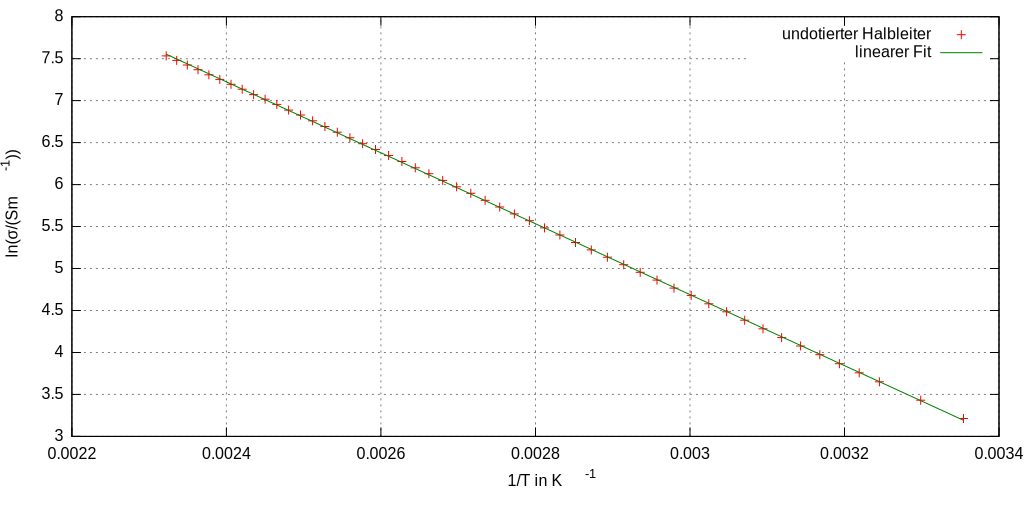
\includegraphics[width=\textwidth]{messwerte/undotiert.pdf}
	\caption{$\ln\left(\unit[\sigma]{/Sm^{-1}} \right)$ über $\frac{1}{T}$ Diagramm mit Fit zur Funktion $f\left(\frac{1}{T}\right)=a\cdot\frac{1}{T}+b$} \label{img:undlogsig}
\end{figure}
Dabei hat sich mittels Methode der kleinsten Quadrate eine Steigung von $a=\unit[-4225,73\,(403)]{K}$ ergeben. Nach Gleichung \ref{eq:logsigma} ist dies $-\frac{E\ix{G}}{2\cdot k\ix{B}}$, also $E\ix{G}=-2\cdot k\ix{B}\cdot a=\unit[0,72828\,(69)]{eV}$.
\subsection{Dotierte Ge-Kristalle}
\subsubsection{Ladungsträgerdichte bei Raumtemperatur}
Als nächstes wurde die Hall-Spannung $U\ix{H}$ in einem p- und einem n-dotierten Germanium-Kristall als Funktion des angelegten Magnetfelds $B$ gemessen, um die Hall-Konstante und daraus die Ladungsträgerkonzentration nach \ref{eq:hall-konst}, beziehungsweise einer Näherung dieser Beziehung, zu bestimmen. In \ref{img:hall-konst} ist $U\ix{H}$ über $B$ aufgetragen und an eine Funktion $U(B)=R\ix{H}\cdot B$ angepasst.
\begin{figure}[H]
	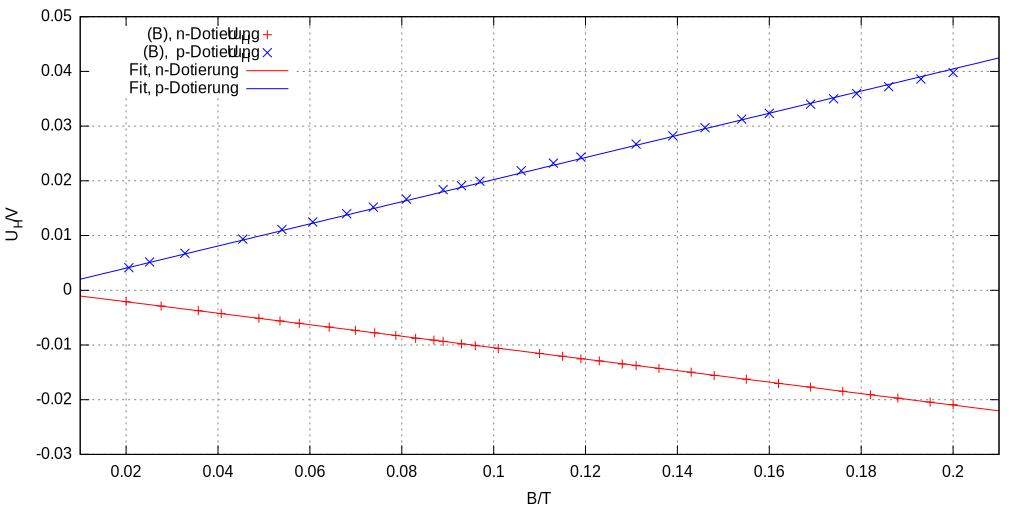
\includegraphics[width=\textwidth]{messwerte/hallkonstanten.pdf}
	\caption{$U\ix{H}$ über $B$ Diagramm mit Fit zur Funktion $U(B)=R\ix{H}\cdot B$} \label{img:hall-konst}
\end{figure}
Dabei hat sich ein Anstieg von $R\ix{H}=\unit[-0,104947\,(46)]{VT^{-1}}$ für die n-dotierte und $R\ix{H}=\unit[0,202243\,(461)]{VT^{-1}}$ für die p-dotierte Probe ergeben.
\subsubsection{Temperaturabhängigkeit der Ladungsträgerdichten}
Nun wurde bei festem Magnetfeld $B$ und Querstrom $I$ die Temperatur der Kristalle variiert, um die Veränderung der Hall-Spannung und damit der Hallkonstante und schließlich der Ladungsträgerkonzentration zu beurteilen. Nach \ref{ch:dot} erwartet man im hohen Temperaturbereich einen Verlauf $\propto \exp\left(-\frac{E\ix{G}}{2\cdot k\ix{B}\cdot T} \right)$, im mittleren Temperaturbereich einen konstanten Verlauf und im niedrigeren Temperaturbereich einen Verlauf $\propto \exp\left(-\frac{E\ix{d}}{2\cdot k\ix{B}\cdot T} \right)$, was sich in der logarithmischen Darstellung von $n$ beziehungsweise $p$ über $\frac{1}{T}$ bemerkbar machen sollte. Diese ist in \ref{img:dotierttemperatur} zu sehen. Tatsächlich sieht man im Bereiche höherer Temperatur einen annähernd linear fallenden Verlauf, der bei niedrigerer Temperatur in ein Plateau über geht. Dies sind jeweils die Bereiche, in denen intrinsische Leitung, beziehungsweise Störstellenerschöpfung auftritt. Die Störstellenreserve lässt sich in unserem Temperaturbereich noch nicht feststellen, da unsere niedrigste Temperatur gerade einmal $\unit[294,85]{K}$ betrug. Jedoch sind die Anstiege in der logarithmischen Darstellung unterschiedlich; man würde erwarten, dass in der intrinsischen Leitung, deren einziger Parameter die Halbleitermaterial-Konstante $E\ix{G}$ ist, bei gleichen Halbleiterrohstoffen gleiche Anstiege zu sehen sind.
\begin{figure}[H]
	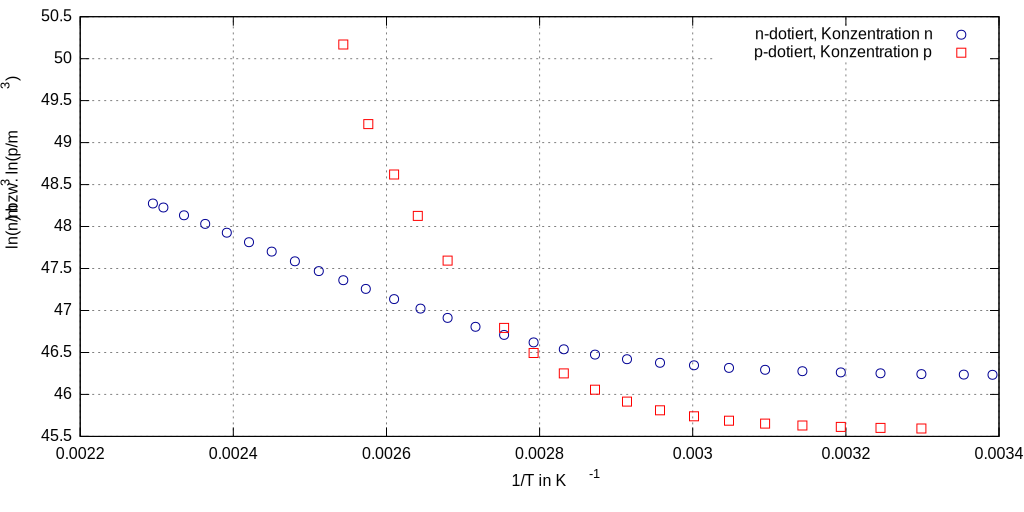
\includegraphics[width=\textwidth]{messwerte/temperaturkonzentration.pdf}
	\caption{$\ln\left(\unit[n]{\cdot m^3}\right)$ über $\frac{1}{T}$ Diagramm} \label{img:dotierttemperatur}
\end{figure}
\subsubsection{Temperaturabhängigkeit der Ladungsträgerbeweglichkeiten}
Wie in \ref{ch:beweg} bereits erläutert und in \ref{img:beweglichkeit} zu sehen, wird die Beweglichkeit der Ladungsträger durch, hauptsächlich 2 Umstände eingeschränkt: Streuung an Störstellen mit Ladungen und an Quasiteilchen von Gitterschwingungen. Für niedrigere Temperaturen erwarten wir somit, bei einer doppelt-logarithmischen Auftragung, einen Anstieg von $\sim\frac{3}{2}$. Andererseits folgt im bereich hoher Temperaturen ein Anstieg $\sim-\frac{3}{2}$ (siehe Gl. (\ref{eq:beweg2}).\\
Der Anstieg der Geraden in \ref{img:mu-n}, welche eine lineare Näherung in einem, unter Vergleich mit \ref{img:beweglichkeit} sinnvollen Bereich darstellt, beträgt $-2,316$. Für \ref{img:mu-p} fanden wir einen Anstieg \mbox{von $-3,322$.} Diese Werte weichen stark von den Erwartungen ab.
\begin{figure}[H]
	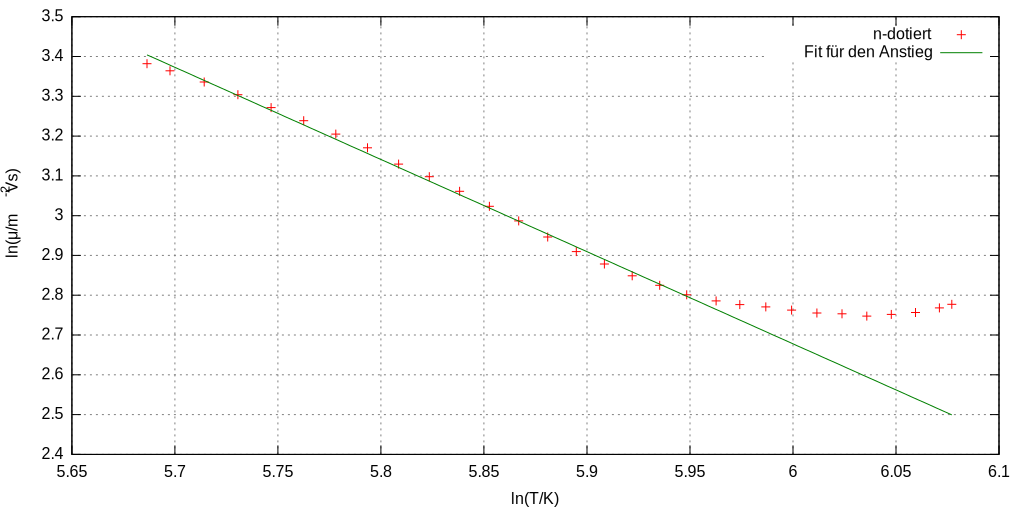
\includegraphics[width=\textwidth]{messwerte/beweglichkeitn.pdf}
	\caption{Logarithmus der Beweglichkeit $\mu\ix{n}$ als Funktion des Logartihmus der Temperatur} \label{img:mu-n}
\end{figure}
\begin{figure}[H]
	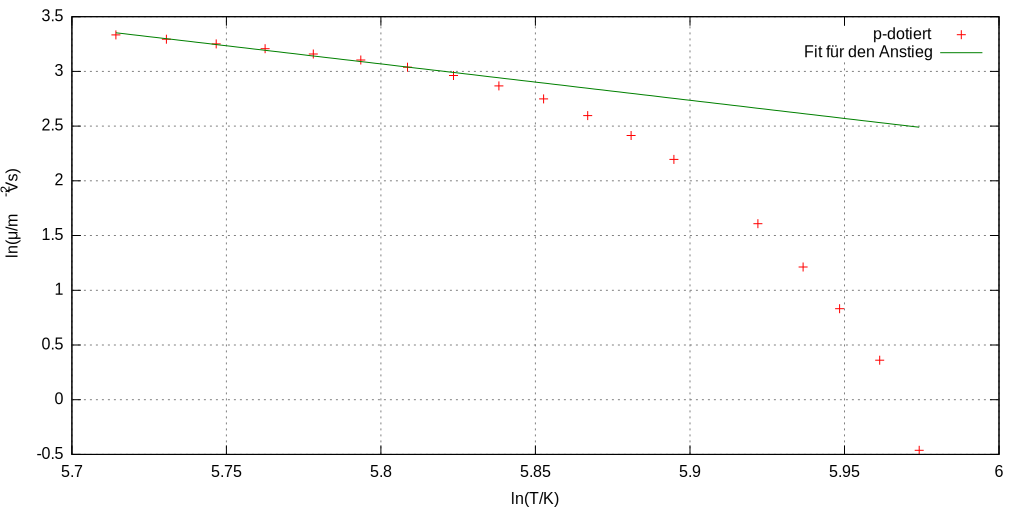
\includegraphics[width=\textwidth]{messwerte/beweglichkeitp.pdf}
	\caption{Logarithmus von $\mu\ix{p}$ über dem Logarithmus von $T$} \label{img:mu-p}
\end{figure}
\section{Quellen}
\begin{itemize}
	\item{\url{http://de.wikipedia.org/wiki/Bandstruktur}\\ Abschn.: Bandstrukturen realer Festkörper}
	\item{Festkörperphysik, Vorlesungsskript zur Vorlesung im WS 1998/1999 und SS 1999; Prof. Dr. Rudolf Gross, Dr. Achim Marx\\
		S.414, Abb. 10.11}
	\item{Festkörperphysik: Einführung in die Grundlagen; H. Ibach, H. Lüth\\
	(Springer-Verlag, Berlin, 1993)\\
		Kap. 12, S.408-423}
	\item{Festkörperphysik, SS 2014; Prof. Dr. Hippler, Prof. Dr. Münzenberg,\\ \mbox{Dr. von der Ehe (geb. Walter)}\\
		Übungsblatt 7, Aufgabe 3}
\end{itemize}\end{document}